\documentclass{beamer}
\usetheme{Madrid}
\usecolortheme{beaver}
\usepackage{tikz}
\usetikzlibrary{calc,arrows.meta,positioning,shapes}
\usepackage{graphicx}
\usepackage[utf8]{inputenc}

\newcommand{\rs}[1]{{\color{red} RS:  #1}}

\newcommand{\cN}{\mathcal{N}}
\newcommand{\cO}{\mathcal{O}}
\newcommand{\bi}{\begin{itemize}}
\newcommand{\ei}{\end{itemize}}

%Information to be included in the title page:
\title[VAE]{String Theory meets Machine Learning\\
	- (Variational) Autoencoder}
\author{Robin Schneider}
\institute{Uppsala University}
\date{November 2020}


\begin{document}
	
\frame{\titlepage}

\begin{frame}
\frametitle{Unsupervised learning}
What is unsupervised learning?
\begin{itemize}
	\item Cluster analysis, anomaly detection, learning latent variables, generating data
	\item Supervised learning is conditional probability $p_\theta (y|X)$, unsupervised is learning true distribution $p_\theta (X) \approx p^*(X)$
	\item Self learning
\ei
\pause
Algorithms
\bi
	\item K-means clustering
	\item Principal component analysis
	\item Generative Adversial Networks (GANs)
	\item (Variational) Autoencoder
	\item (Persistent homology)
\end{itemize}
\end{frame}

\begin{frame}
\frametitle{Autoencoders}
\begin{figure}
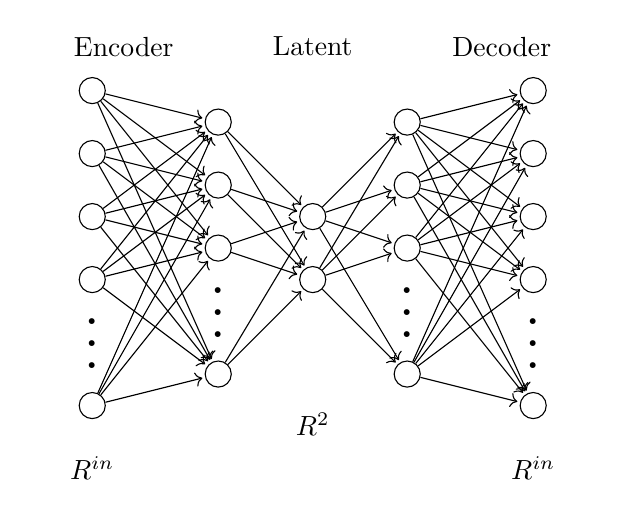
\begin{tikzpicture}[shorten >=1pt,node distance=2cm,scale=0.8]
\tikzset{
	annot/.style={
		text width=4em,
		text centered,		
	}
}
\tikzset{%
	every neuron/.style={
		circle,
		draw,
	},
	neuron missing/.style={
		draw=none, 
		scale=2,
		text height=0.333cm,
		execute at begin node=\color{black}$\vdots$
	},
}


% Neuron Nodes
% Input
\foreach \m/\l [count=\y] in {1,2,3,4,missing,5}
\node [every neuron/.try, neuron \m/.try] (I-\m) at (1,6.5-\y) {};%
\node [annot] (Input) at (1.5,6.2) {Encoder};%
\node [annot] (IR) at (1,-0.5) {$\mathbb{R}^{in}$};%

%H1
\foreach \m/\l [count=\y] in {1,2,3,missing,4}
\node [every neuron/.try, neuron \m/.try] (H1-\m) at (3,6-\y) {};

%L
\foreach \m/\l [count=\y] in {1,2}
\node [every neuron/.try, neuron \m/.try] (L-\m) at (4.5,4.5-\y) {};%
\node [annot] (L) at (4.5,0.2) {$\mathbb{R}^{2}$};%
\node [annot] (LH) at (4.5,6.2) {Latent};	

%H2
\foreach \m/\l [count=\y] in {1,2,3,missing,4}
\node [every neuron/.try, neuron \m/.try] (H2-\m) at (6,6-\y) {};


%O1
\foreach \m/\l [count=\y] in {1,2,3,4,missing,5}
\node [every neuron/.try, neuron \m/.try] (O-\m) at (8,6.5-\y) {};%
\node [annot] (Iutput) at (7.5,6.2) {Decoder};%
\node [annot] (OR) at (8,-0.5) {$\mathbb{R}^{in}$};%		

% Connecting lines
\foreach \i in {1,2,3,4,5}
\foreach \j in {1,2,3,4}
\draw [->] (I-\i) -- (H1-\j);
\foreach \i in {1,2,3,4}
\foreach \j in {1,2}
\draw [->] (H1-\i) -- (L-\j);
\foreach \i in {1,2}
\foreach \j in {1,2,3,4}
\draw [->] (L-\i) -- (H2-\j);
\foreach \i in {1,2,3,4}
\foreach \j in {1,2,3,4,5}
\draw [->] (H2-\i) -- (O-\j);
\end{tikzpicture}
\caption{ \it A fully connected autoencoder with two latent dimensions.}
\end{figure}
\end{frame}

\begin{frame}
\frametitle{Applications}
What are autoencoders good for?
\bi
\item Data denoising
\item Data compression to latent dimension
\item Data visualization (clustering)
\item Anomaly detection
\ei
Let's go back to out favourite data set MNIST.
\end{frame}

\begin{frame}
\frametitle{MNIST autoencoder}
\begin{figure}
\begin{minipage}{0.45\linewidth}
	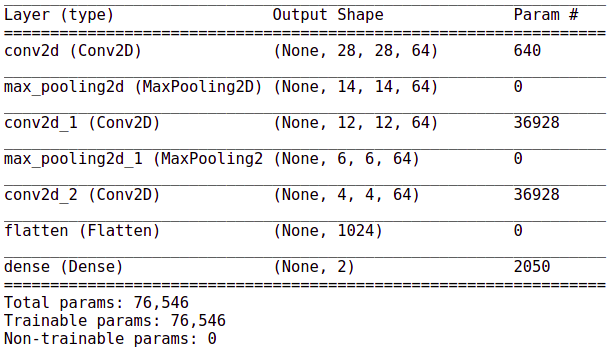
\includegraphics[scale=0.24]{mnist_ae_encoder.png}
\end{minipage}
\begin{minipage}{0.45\linewidth}
	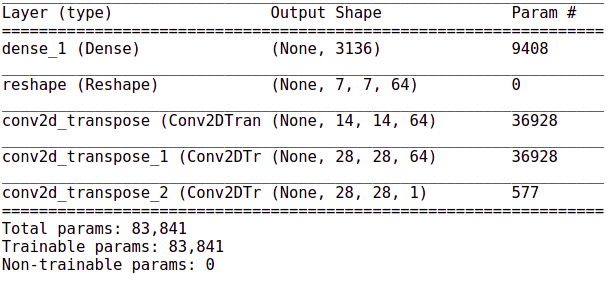
\includegraphics[scale=0.24]{mnist_ae_decoder.png}
\end{minipage}
	\caption{\it Neural network architecture for encoder and decoder applied to MNIST data set with two latent dimensions.}
\end{figure}
\end{frame}

\begin{frame}
\frametitle{MNIST denoising}
\begin{figure}
	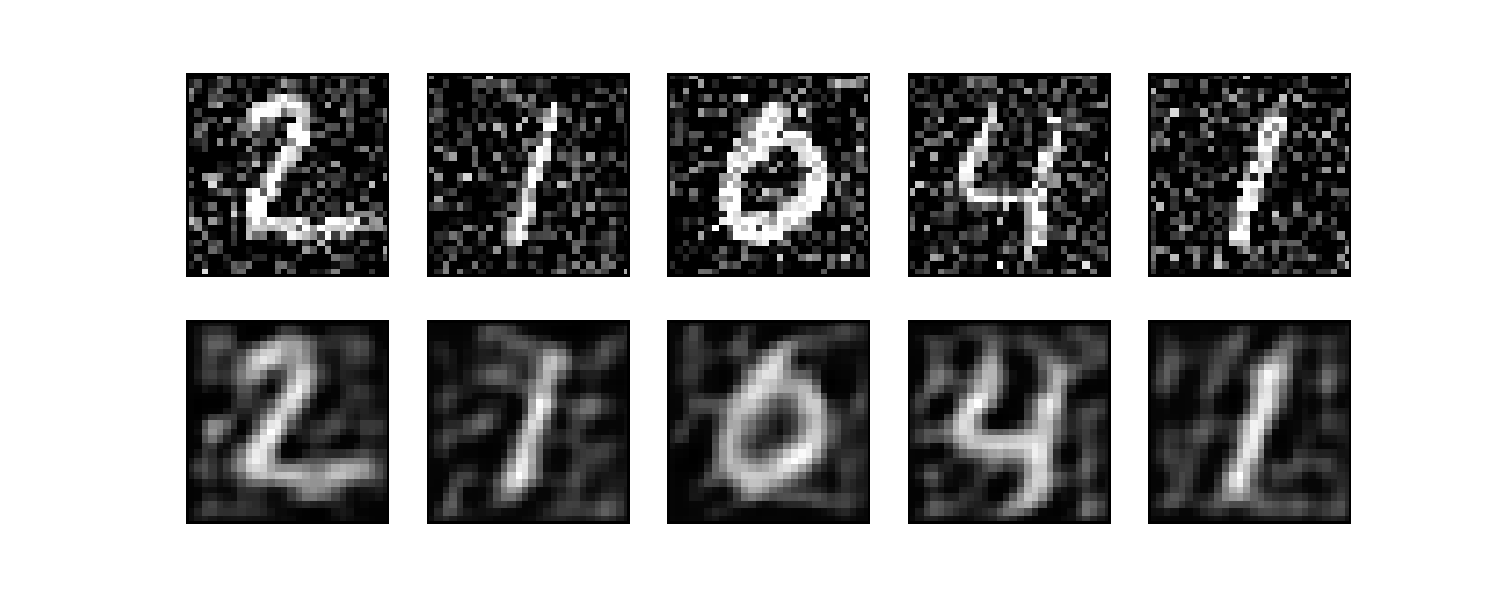
\includegraphics[scale=0.5]{ae_denoised.pdf}
	\caption{\it On the top row noisy hand written numbers of the MNIST data set. On the bottom row the denoised pictures after running through an auto encoder.}
\end{figure}
\end{frame}

\begin{frame}
\frametitle{MNIST compression}
\begin{figure}
	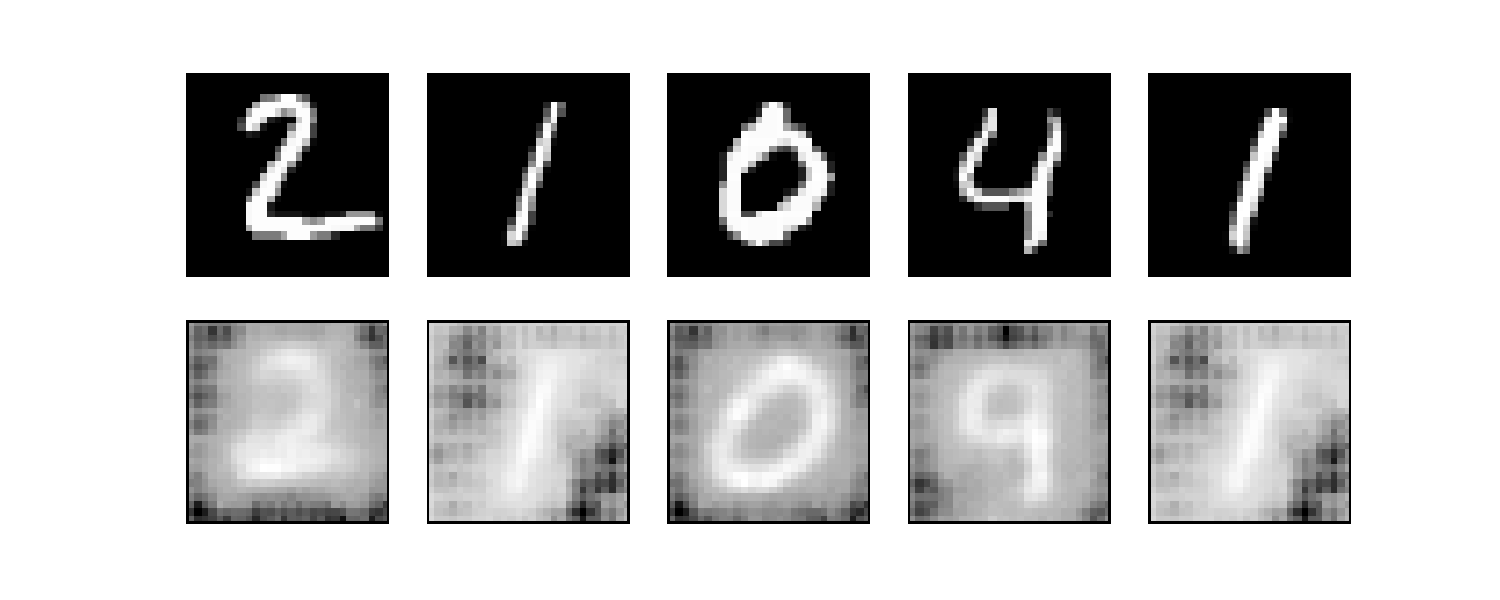
\includegraphics[scale=0.5]{ae_compression.pdf}
	\caption{\it (De-)compression of MNIST images to two latent dimensions. On the top row five hand written digits and on the bottom after running through the encoder.}
\end{figure}
\end{frame}

\begin{frame}
\frametitle{MNIST visualization}
\begin{figure}
\begin{minipage}{0.45\linewidth}
	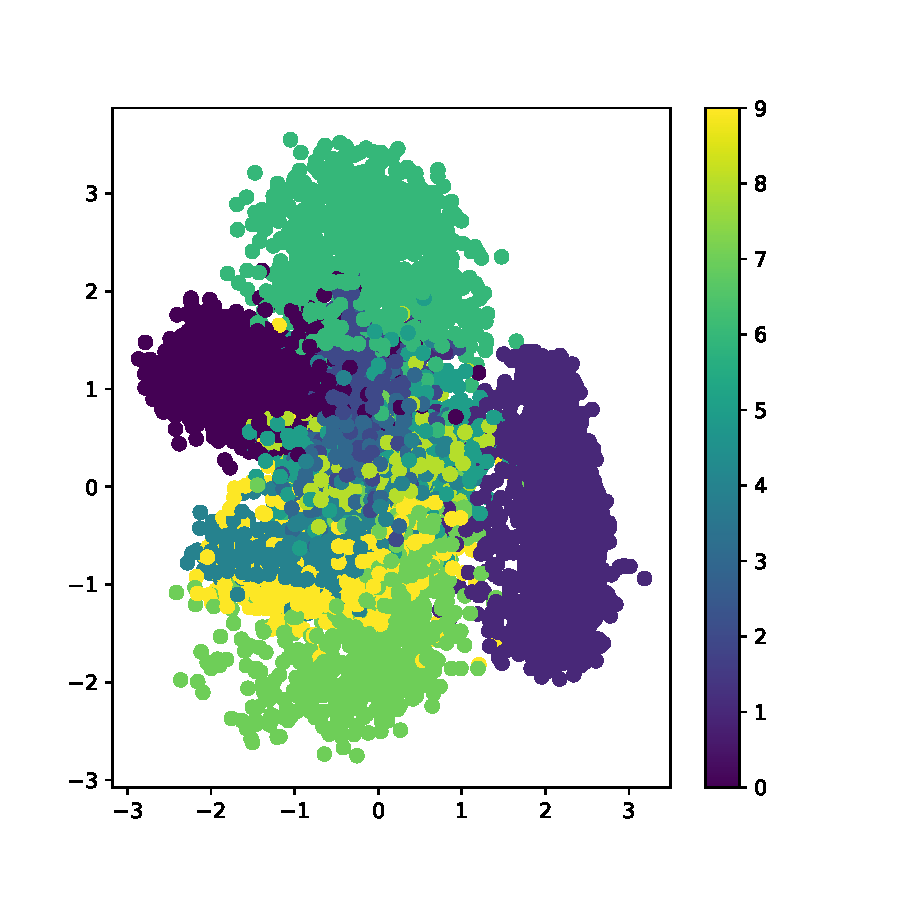
\includegraphics[scale=0.4]{ae_encoder.pdf}
\end{minipage}
\begin{minipage}{0.45\linewidth}
	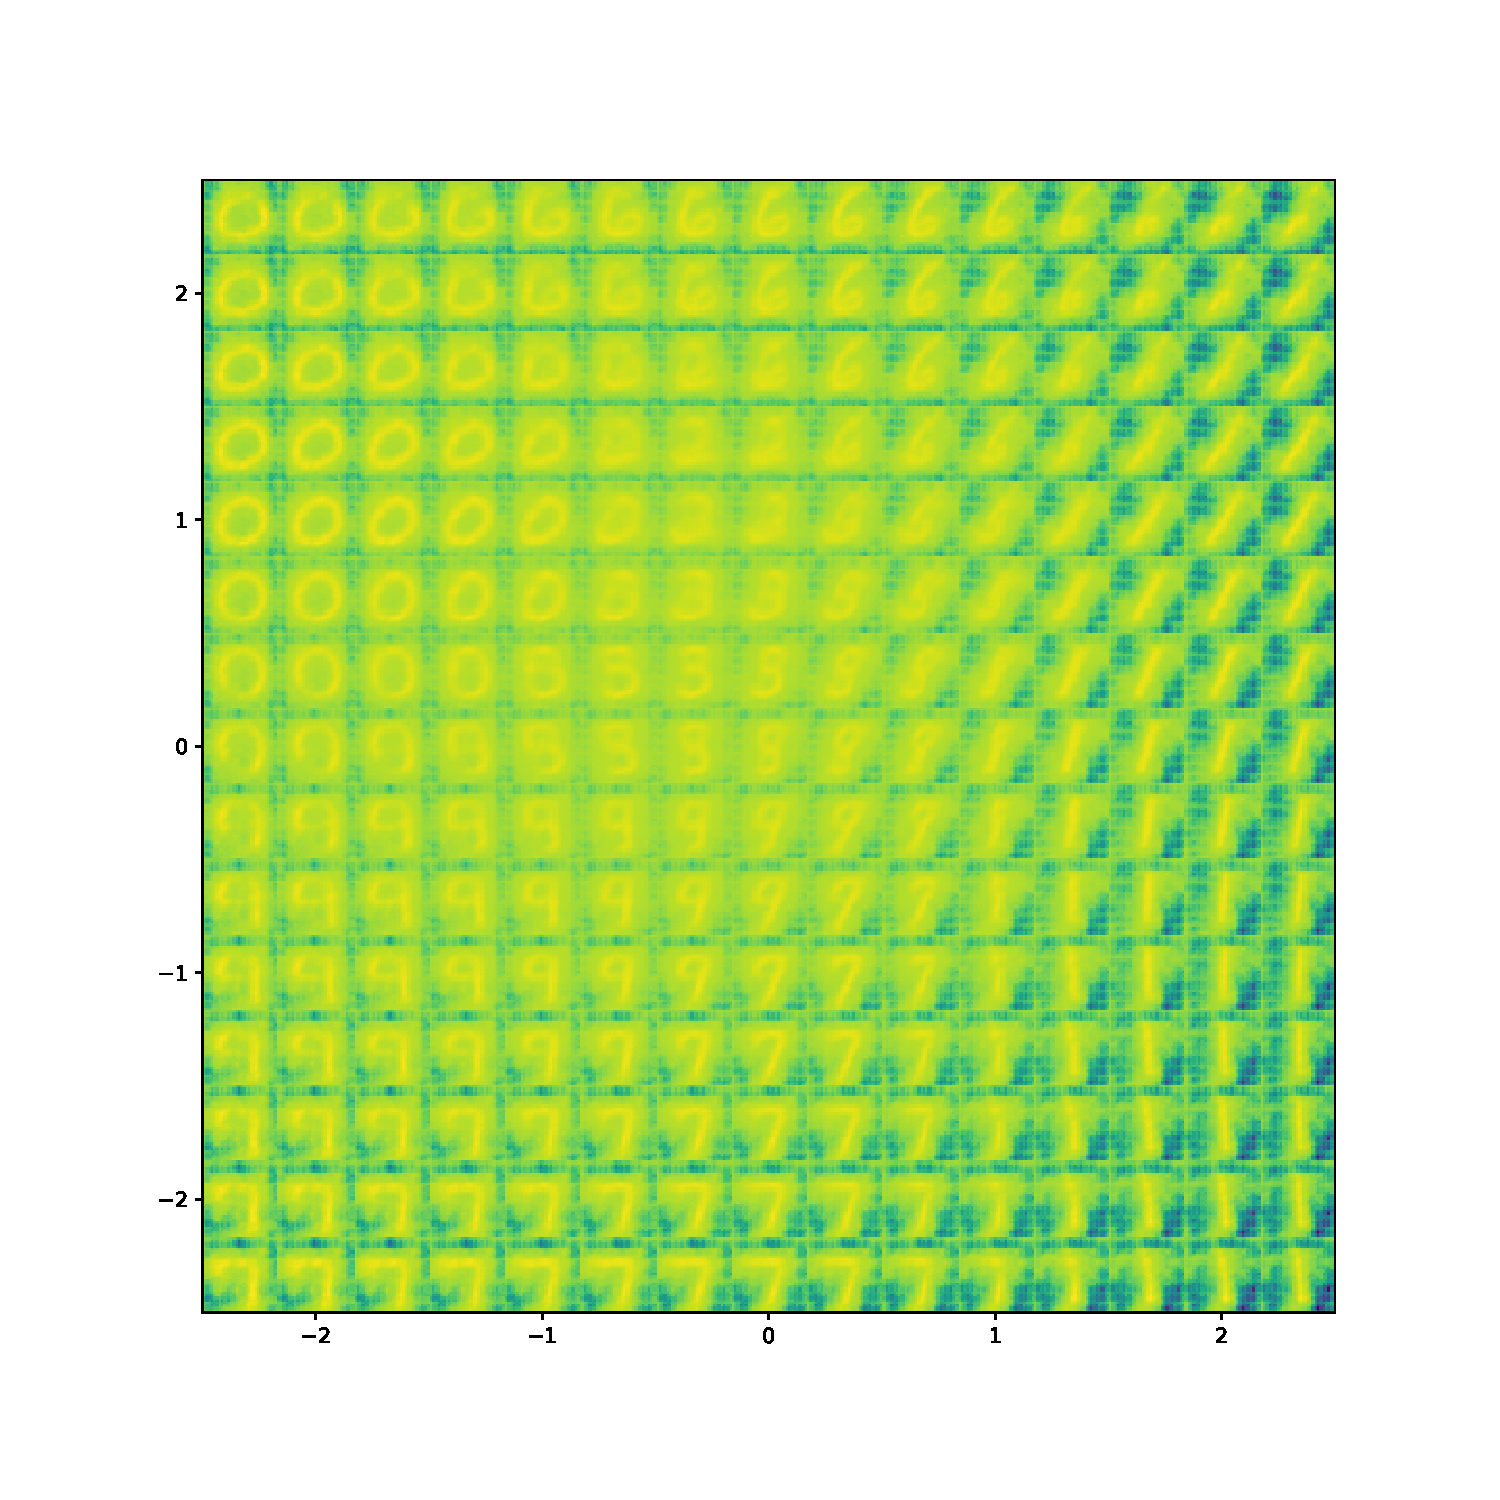
\includegraphics[scale=0.24]{ae_decoder.pdf}
\end{minipage}
\caption{\it On the left clustering of MNIST digits to two latent dimensions via encoder, on the right decoded images of samples from the two latent dimensions.}
\end{figure}
\end{frame}

\begin{frame}
\frametitle{Standard Like Model}
Heterotic string compactification with three ingredients {\color{blue} [1106.4804,1202.1757,1307.4787]}.
\begin{enumerate}
\item Calabi Yau manifold $M$. \item Line bundle sum $V = \otimes_{a=1}^5 L_a$. \item Freely acting discrete symmetry $\Gamma$ for Wilson line.
\end{enumerate}
For example:
\begin{align}
	\mathcal{M}_{5302} =  \left[
	\begin{array}{c||ccc}
	1 & 0 & 1 & 1 \\
	1 & 0 & 1 & 1 \\
	1 & 1 & 1 & 0 \\
	1 & 1 & 1 & 0 \\
	1 & 1 & 0 & 1 \\
	1 & 1 & 0 & 1
	\end{array}
	\right]^{6,30}_{-48} \text{ and }  V = \left[\begin{array}{ccccc}
	-1 & -1 & 0 & 1 & 1 \\
	-1& -1&  1&  0&  1\\
	-1& -1&  1&  1&  0\\
	1& 1&  0&  0& -2\\
	1& 1&  -2&  1&  -1\\
	1& 1&  0&  -2&  0
	\end{array}\right]\nonumber 
\end{align}
and $|\Gamma| = 4$. There are a total of 17329 such models.
\end{frame}

\begin{frame}
\frametitle{SLM autoencoder}
\begin{figure}
	\begin{minipage}{0.45\linewidth}
		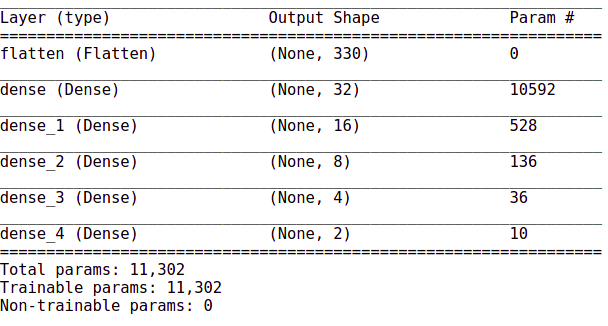
\includegraphics[scale=0.24]{ae_encoder_net.png}
	\end{minipage}
	\begin{minipage}{0.45\linewidth}
		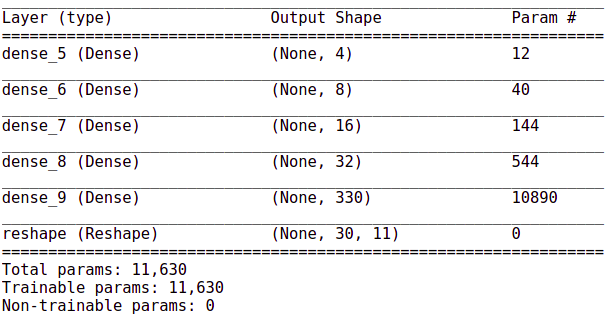
\includegraphics[scale=0.24]{ae_decoder_net.png}
	\end{minipage}
	\caption{\it Neural network architecture for encoder and decoder applied to SLM data set with two latent dimensions.}
\end{figure}
\end{frame}

\begin{frame}
\frametitle{SLM visualization}
\begin{figure}
	\begin{minipage}{0.48\linewidth}
	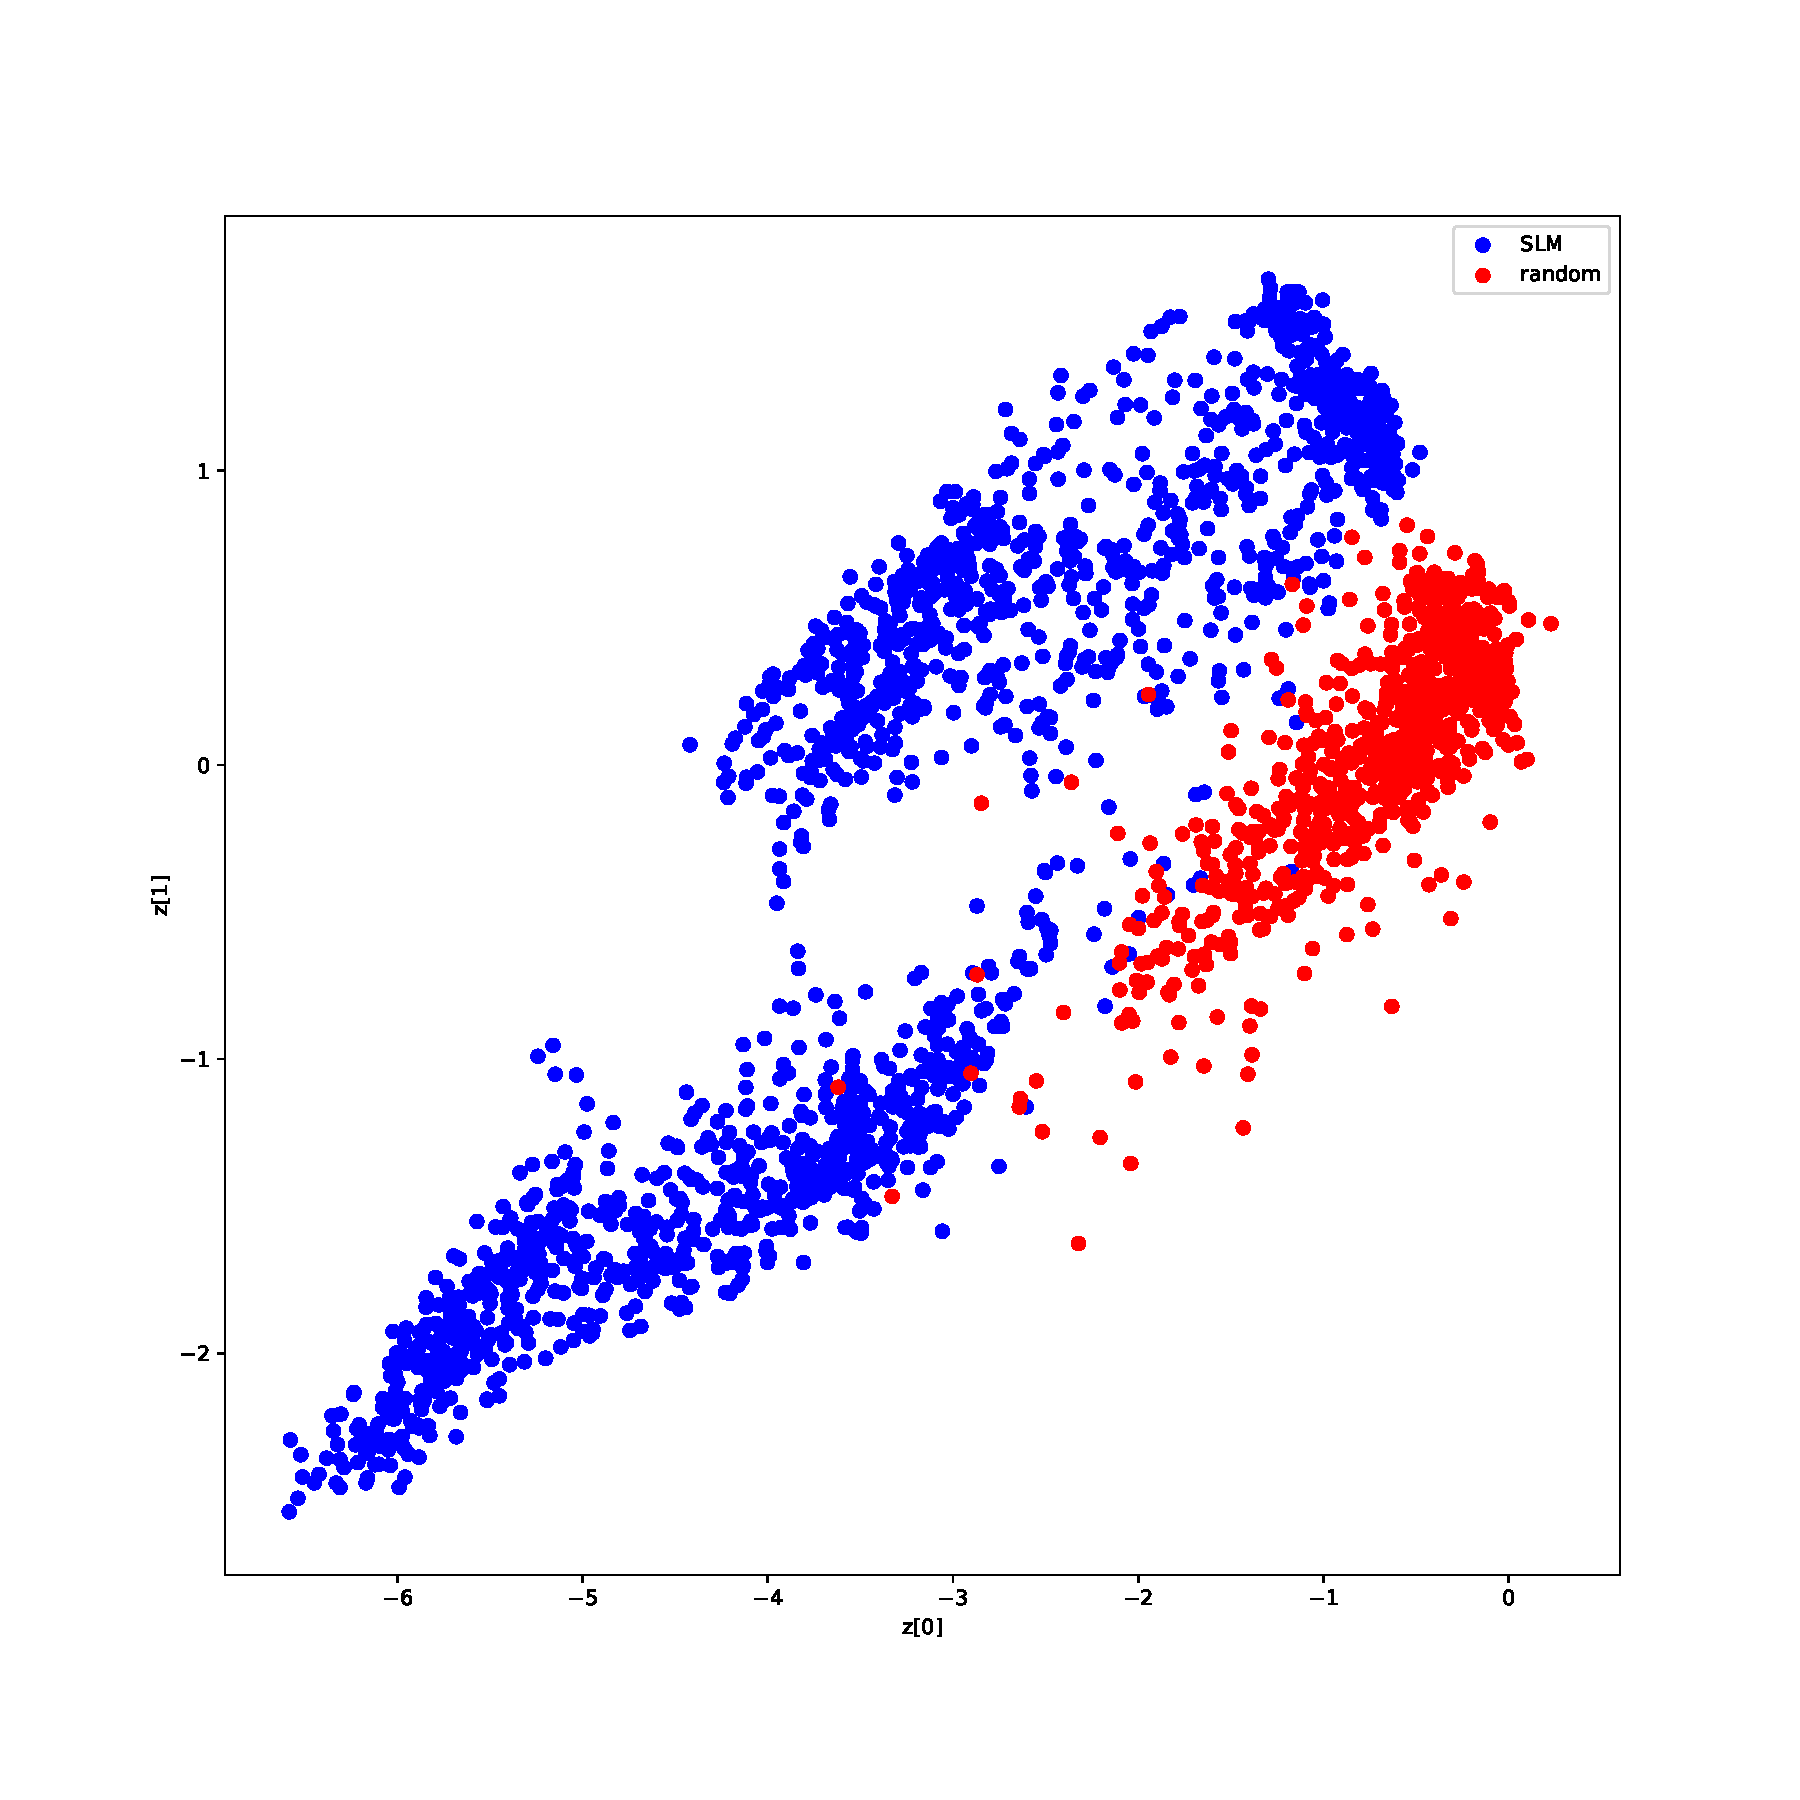
\includegraphics[scale=0.21]{ae_slm_norm.pdf}
	\end{minipage}
	\begin{minipage}{0.48\linewidth}
		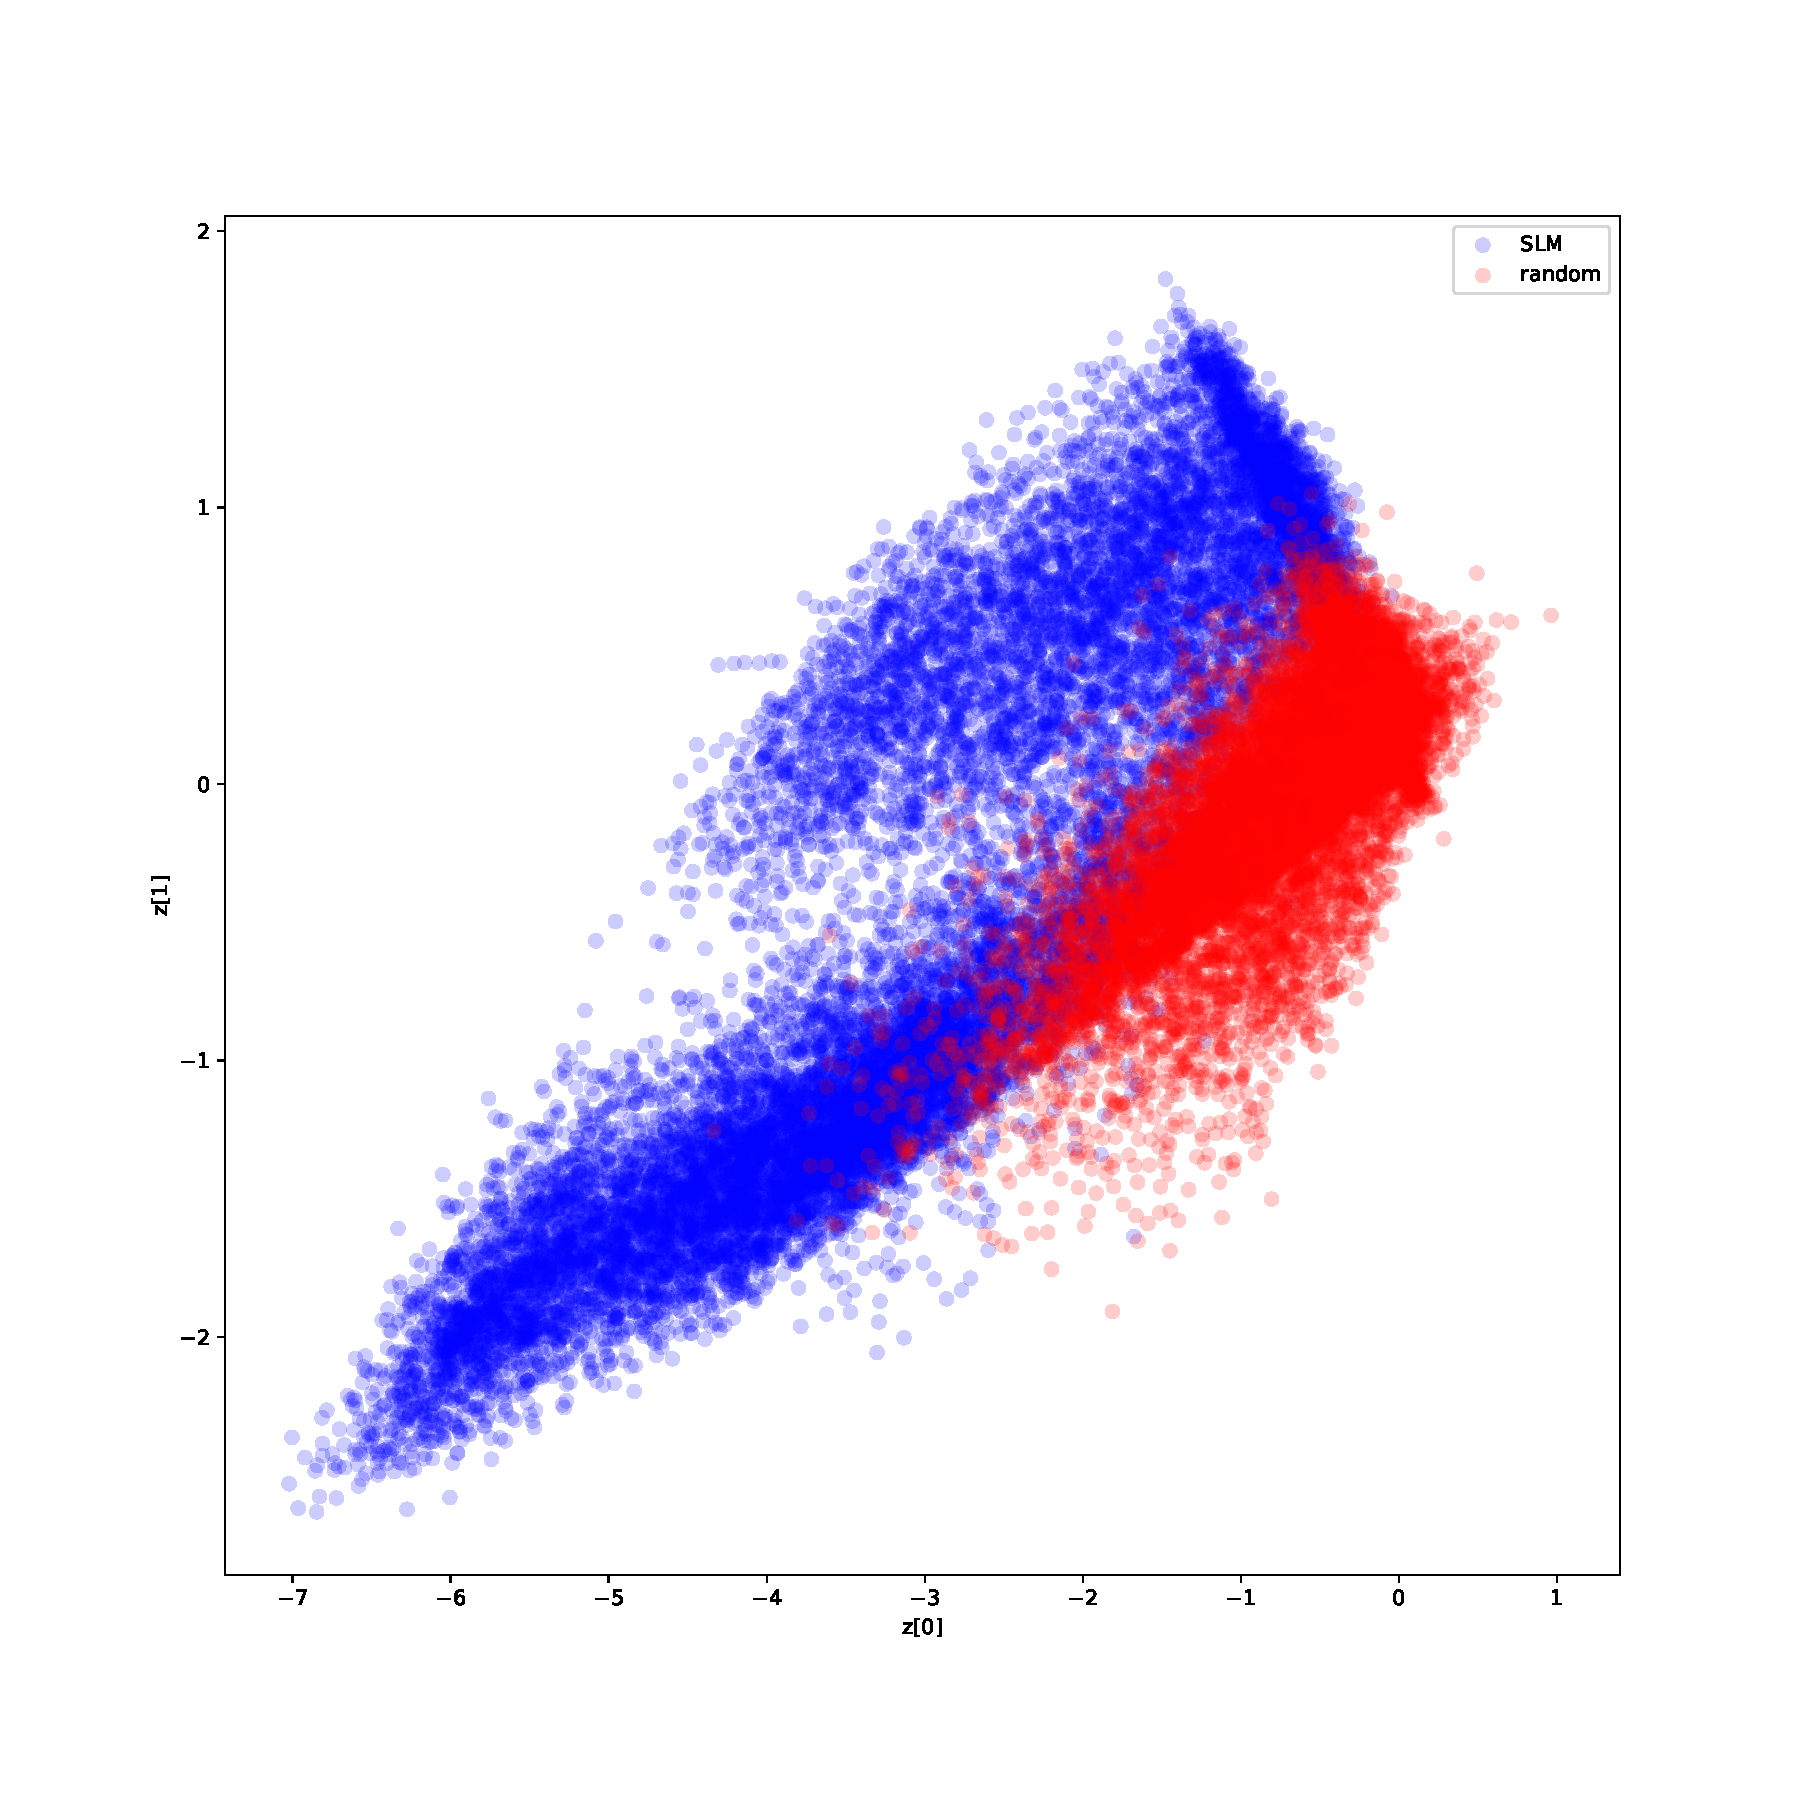
\includegraphics[scale=0.21]{ae_slm_all.pdf}
	\end{minipage}
	\caption{\it Image of clustered Standard like models. First investigated in {\color{blue}[2003.13339]}. To the left with norm $V<5$. To the right all SLMs.}
\end{figure}
\end{frame}

%\begin{frame}
%\frametitle{K-means clustering}
%add something
%\end{frame}

\begin{frame}
\frametitle{Variational Autoencoders}
Variational Autoencoders are generative modeling $p_\theta(X|z)$. They
\bi
\item combine stochastic gradient descent and Bayesian inference into deep generative models {\color{blue} [1312.6114,1401.4082,1906.02691]},
\item are with GANs the most popular generative model,
\item are used in Physics, e.g. at CERN or in astronomy.
\ei
\pause
\vspace{0.2cm} 
\textbf{Starting point:} Assume there are some latent variables $z$ controlling your data $X$. Take a deterministic function (decoder) $f(\theta): z \rightarrow X$. 

Here $z$ is a random variable. Then $f(z, \theta)$ also becomes random.
\end{frame}


\begin{frame}
\frametitle{Probability Density Function}
Assume that $p(z)$ and $p_\theta(X|z)$ follow some PDF we can then marginalize
\begin{align}
	p_\theta(X) = \int p_\theta(X,z) dz = \int p_\theta(X|z) p(z) dz
\end{align}
This integral is often intractable, see e.g {\color{blue}[1601.00670]}.
% See e.g. [1601.00670] why intractable

\pause
We take
\begin{align}
	p_\theta(X|z) = \cN(X|\mu = f(z,\theta), \sigma^2)
\end{align}
and introduce an approximation to posterior $p_\theta(z|X)$, an inference model 
\begin{align}
q_\phi(z|x) = \cN(X|\mu, \sigma^2), \text{ with } (\mu, \sigma^2) \sim h(X, \phi)
\end{align}
Assume there exists no single good interpretation of $z$, hence the prior is
\begin{align}
	p(z) =  \cN(0,I).
\end{align}
\end{frame}

\begin{frame}
\frametitle{ELBO and KL}
Want to maximize $\log p_\theta (X)$:
\begin{align}
	 \mathbb{E}_{q_\phi (z|X)} [\log p_\theta (X)] &= \mathbb{E}_{q_\phi (z|X)} \left[\log \frac{p_\theta (X,z)}{p_\theta (z|X)} \right] \nonumber \\ %\log p_\theta (X) &=
	& =  \mathbb{E}_{q_\phi (z|X)} \left[\log \frac{p_\theta (X,z)}{q_\phi (z|X)} \frac{q_\phi (z|X)}{p_\theta (z|X)} \right] \nonumber \\
	& =  \underbrace{\mathbb{E}_{q_\phi (z|X)} \left[\log \frac{p_\theta (X,z)}{q_\phi (z|X)}\right] }_{:= \mathcal{L}_{\theta, \phi} (x)} + \underbrace{\mathbb{E}_{q_\phi (z|X)} \left[\log \frac{q_\phi (z|X)}{p_\theta (z|X)}\right] }_{:= D_{KL} (q_\phi (z|X) || p_\theta (z|X))}
\end{align}

\pause
First term is Evidence Lower BOund (ELBO), second term is Kullback-Leibler divergence, which measures the relative 'difference' between two probability distributions (always positive)\footnote{Recall entropy:
$
	H = - \sum_{i=1}^{N} p(x_i) \cdot \log p(x_i)
$}. Want to \textbf{maximize} ELBO 1. maximizes log likelihood, 2. minimize KL divergence.
\end{frame}

\begin{frame}
\frametitle{Optimizing and Monte Carlo sampling}
Gradient descent on ELBO
\begin{align}
	\nabla_\theta \mathcal{L}_{\theta, \phi} &= \nabla_\theta \mathbb{E}_{q_\phi (z|X)} \left[\log \frac{p_\theta (X,z)}{q_\phi (z|X)}\right] \nonumber \\
	& \simeq \nabla_\theta \log p_\theta (X,z)
\end{align}
works just fine. However, $\nabla_\phi \mathcal{L}_{\theta, \phi}$ more tricky, since we can't pull $\nabla_\phi$ into $\mathbb{E}_{q_\phi (z|X)}$.

\pause
\textbf{Solution:} Use reparametrization trick. Generate samples from $z \sim q_\phi (z|x)$. Reparametrize $z = g(\epsilon,X,\phi)$, where $\epsilon$ has independent distribution, e.g. $p(\epsilon) = \cN (0,1)$. Then $\mathbb{E}_{q_\phi (X)} = \mathbb{E}_{p(\epsilon)}$ and we get a new Monte Carlo estimator
\begin{align}
\nabla_\phi \mathcal{L}_{\theta, \phi} &= \nabla_\phi \mathbb{E}_{p(\epsilon)} = \mathbb{E}_{p(\epsilon)} \left[ \nabla_\phi\log \frac{p_\theta (X,z)}{q_\phi (z|X)} \right] \nonumber \\
& = \nabla_\phi \mathbb{E}_{p(\epsilon)}  \left[ \log p_\theta(X|z) +  \log \frac{p(z)}{q_\phi (z|X)}\right]
\end{align}
\end{frame}

\begin{frame}
\frametitle{KL divergence}

How does the KL divergence for two Gaussians look like?
\begin{align}
	D_{KL} (\cN_0 || \cN_1) &= \frac{1}{2} \bigg( \text{tr} ( \Sigma_1^{-1} \Sigma_0) + (\mu_1 - \mu_0)^T \Sigma_1^{-1} (\mu_1 - \mu) \nonumber  \\
	& \qquad \qquad   - k + \ln \left[ \frac{\det \Sigma_1}{\det \Sigma_0}\right] \bigg)
\end{align}
Hence, for $k=2$ latent dimensions and $\cN_0 = q_\phi (z|X) = \cN (\mu_\phi, \sigma_\phi) $ and $\cN_1 = p (z) = \cN(0,I)$, we simplify to KL loss
\begin{align}
	J_{KL} =  \sigma^2_\phi + \mu_\phi^2 - 1 - \log(\sigma^2_\phi)
\end{align}
In total:
\begin{align}
 J = J_{\text{cross entropy}} + J_{KL} 
\end{align}


%\textbf{Final thoughts:} Reconstruction loss pulls away, KL pulls together.
\end{frame}

\begin{frame}
\frametitle{VAE}
\begin{figure}
	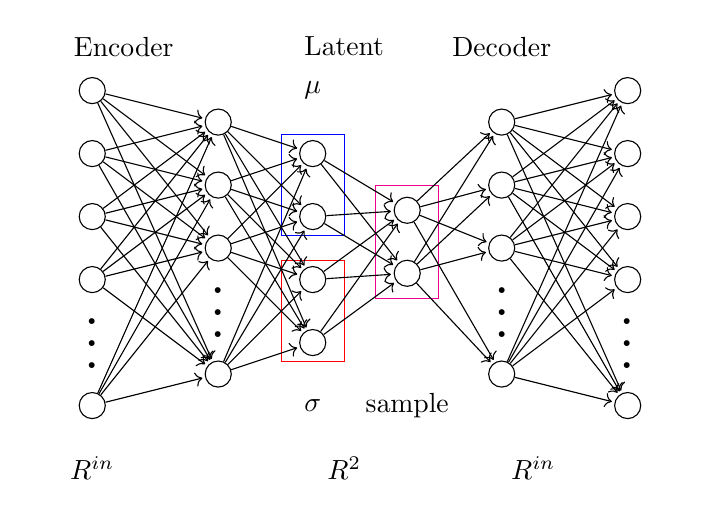
\begin{tikzpicture}[shorten >=1pt,node distance=2cm,scale=0.8]
	\tikzset{
		annot/.style={
			text width=4em,
			text centered,		
		}
	}
	\tikzset{%
		every neuron/.style={
			circle,
			draw,
		},
		neuron missing/.style={
			draw=none, 
			scale=2,
			text height=0.333cm,
			execute at begin node=\color{black}$\vdots$
		},
	}
	
	
	% Neuron Nodes
	% Input
	\foreach \m/\l [count=\y] in {1,2,3,4,missing,5}
	\node [every neuron/.try, neuron \m/.try] (I-\m) at (1,6.5-\y) {};%
	\node [annot] (Input) at (1.5,6.2) {Encoder};%
	\node [annot] (IR) at (1,-0.5) {$\mathbb{R}^{in}$};%
	
	%H1
	\foreach \m/\l [count=\y] in {1,2,3,missing,4}
	\node [every neuron/.try, neuron \m/.try] (H1-\m) at (3,6-\y) {};
	
	%L1, sigma
	\foreach \m/\l [count=\y] in {1,2}
	\node [every neuron/.try, neuron \m/.try] (L1-\m) at (4.5,5.5-\y) {};%
	% mu
	\foreach \m/\l [count=\y] in {1,2}
	\node [every neuron/.try, neuron \m/.try] (L2-\m) at (4.5,3.5-\y) {};%
	
	\draw[solid, color=red] (4,1.2) rectangle (5,2.8);
	\draw[solid, color=blue] (4,3.2) rectangle (5,4.8);
	\draw[solid, color=magenta] (5.5,2.2) rectangle (6.5,4);
	
	\node [annot] (mu) at (4.5,5.5) {$\mu$};%
	\node [annot] (sigma) at (4.5,0.5) {$\sigma$};%
	\node [annot] (sample) at (6,0.5) {sample};%
	
	
	\node [annot] (L) at (5,-0.5) {$\mathbb{R}^{2}$};%
	\node [annot] (LH) at (5,6.2) {Latent};	
	
	%S1 sample
	\foreach \m/\l [count=\y] in {1,2}
	\node [every neuron/.try, neuron \m/.try] (S-\m) at (6,4.6-\y) {};
	
	%H2
	\foreach \m/\l [count=\y] in {1,2,3,missing,4}
	\node [every neuron/.try, neuron \m/.try] (H2-\m) at (7.5,6-\y) {};
	
	
	%O1
	\foreach \m/\l [count=\y] in {1,2,3,4,missing,5}
	\node [every neuron/.try, neuron \m/.try] (O-\m) at (9.5,6.5-\y) {};%
	\node [annot] (Iutput) at (7.5,6.2) {Decoder};%
	\node [annot] (OR) at (8,-0.5) {$\mathbb{R}^{in}$};%		
	
	% Connecting lines
	\foreach \i in {1,2,3,4,5}
	\foreach \j in {1,2,3,4}
	\draw [->] (I-\i) -- (H1-\j);
	\foreach \i in {1,2,3,4}
	\foreach \j in {1,2}
	\draw [->] (H1-\i) -- (L1-\j);
	\foreach \i in {1,2,3,4}
	\foreach \j in {1,2}
	\draw [->] (H1-\i) -- (L2-\j);
	\foreach \i in {1,2}
	\foreach \j in {1,2}
	\draw [->] (L1-\i) -- (S-\j);
	\foreach \i in {1,2}
	\foreach \j in {1,2}
	\draw [->] (L2-\i) -- (S-\j);
	\foreach \i in {1,2}
	\foreach \j in {1,2,3,4}
	\draw [->] (S-\i) -- (H2-\j);
	\foreach \i in {1,2,3,4}
	\foreach \j in {1,2,3,4,5}
	\draw [->] (H2-\i) -- (O-\j);
	\end{tikzpicture}
	\caption{\it A fully connected Variational Autoencoder with two latent dimensions.}
\end{figure}
\end{frame}

\begin{frame}
\frametitle{VAE MNIST architecture}
\begin{figure}
	\begin{minipage}{0.45\linewidth}
		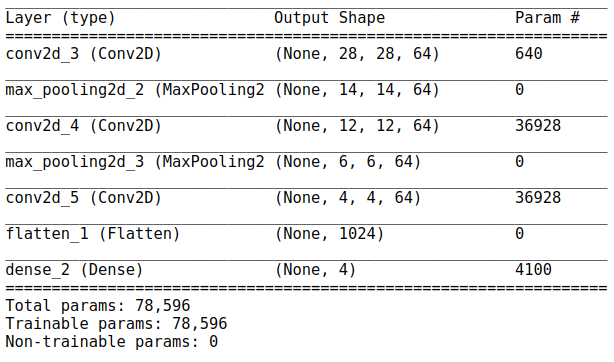
\includegraphics[scale=0.26]{mnist_vae_encoder.png}
	\end{minipage}
	\begin{minipage}{0.45\linewidth}
		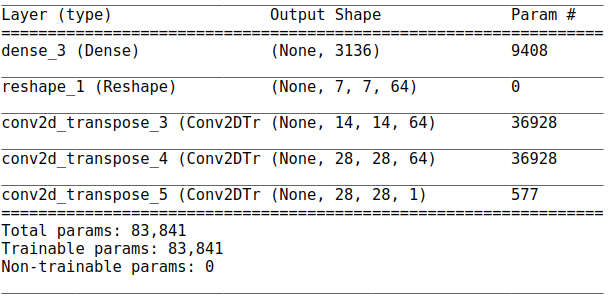
\includegraphics[scale=0.26]{mnist_vae_decoder.png}
	\end{minipage}
	\caption{\it Architecture of encoder and decoder of the VAE.}
\end{figure}
\end{frame}

\begin{frame}
\frametitle{VAE MNIST visualization}
\begin{figure}
	\begin{minipage}{0.45\linewidth}
	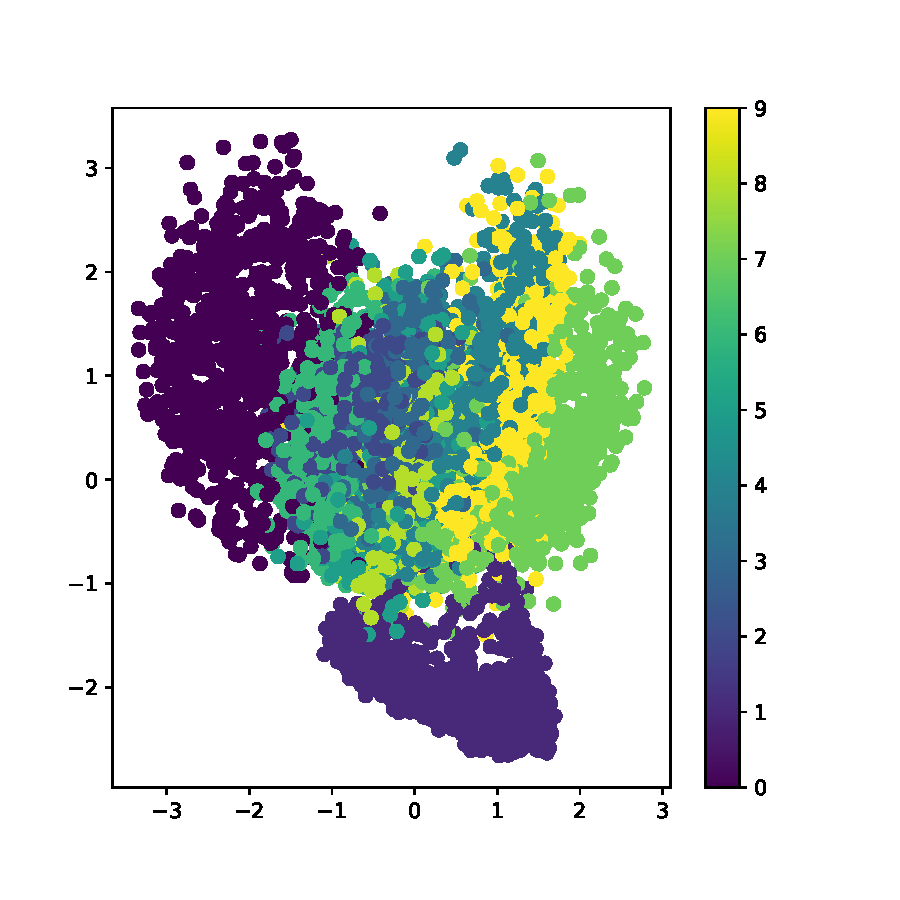
\includegraphics[scale=0.42]{vae_encoder.pdf}
\end{minipage}
	\begin{minipage}{0.45\linewidth}
		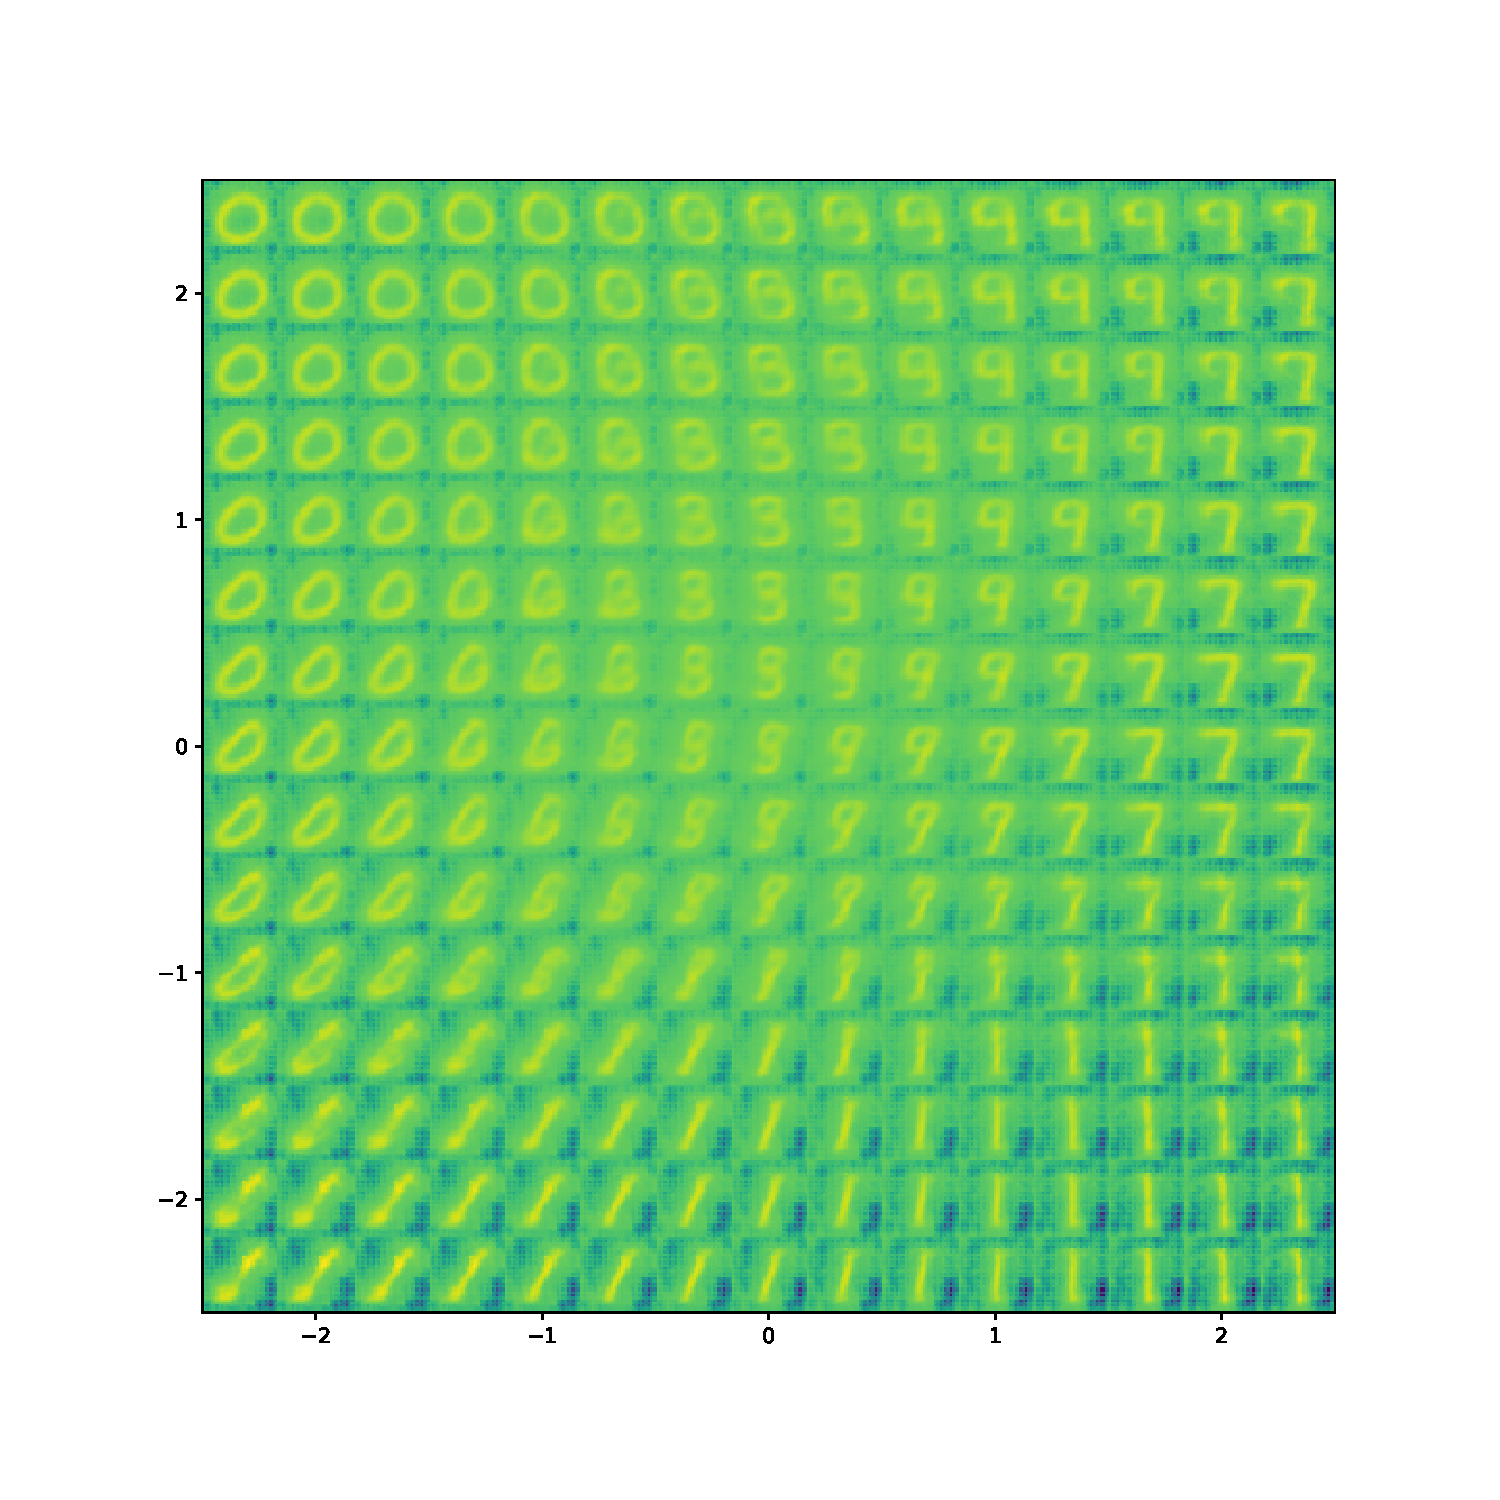
\includegraphics[scale=0.24]{vae_decoder.pdf}
	\end{minipage}
	\caption{\it On the left clustering of MNIST digits to two latent dimensions via encoder, on the right decoded images of samples from the two latent dimensions.}
\end{figure}
\end{frame}

\begin{frame}
\frametitle{VAE SLM visualization}
\begin{figure}
	\begin{minipage}{0.48\linewidth}
		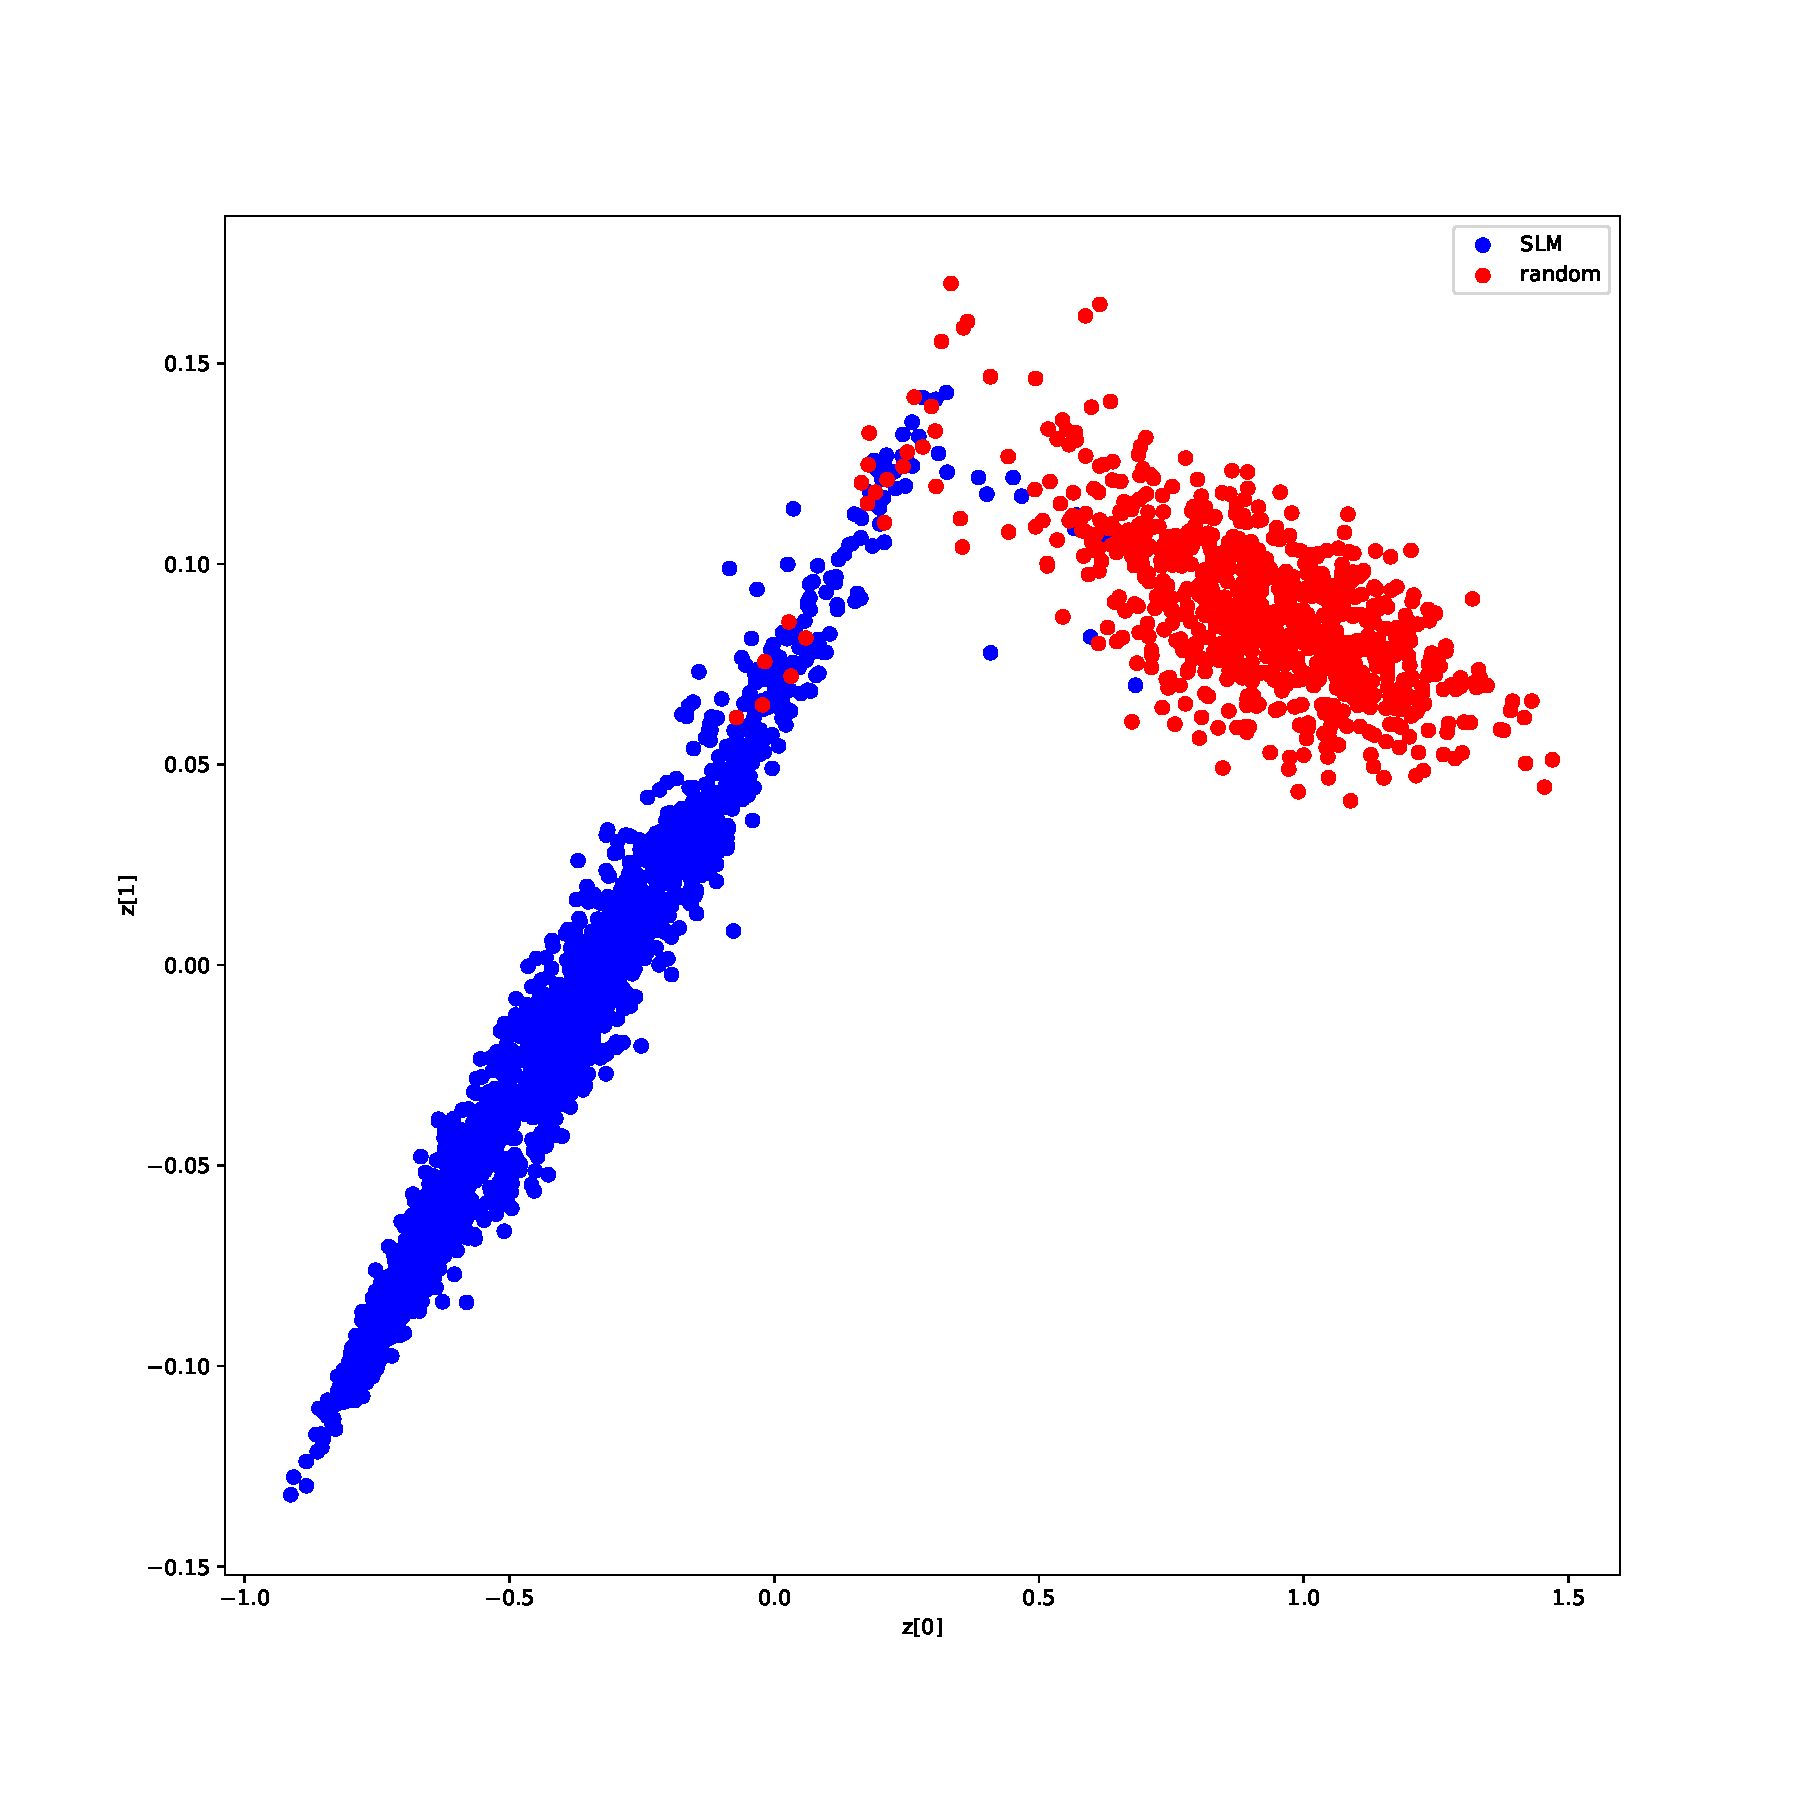
\includegraphics[scale=0.21]{vae_slm_norm.pdf}
	\end{minipage}
	\begin{minipage}{0.48\linewidth}
		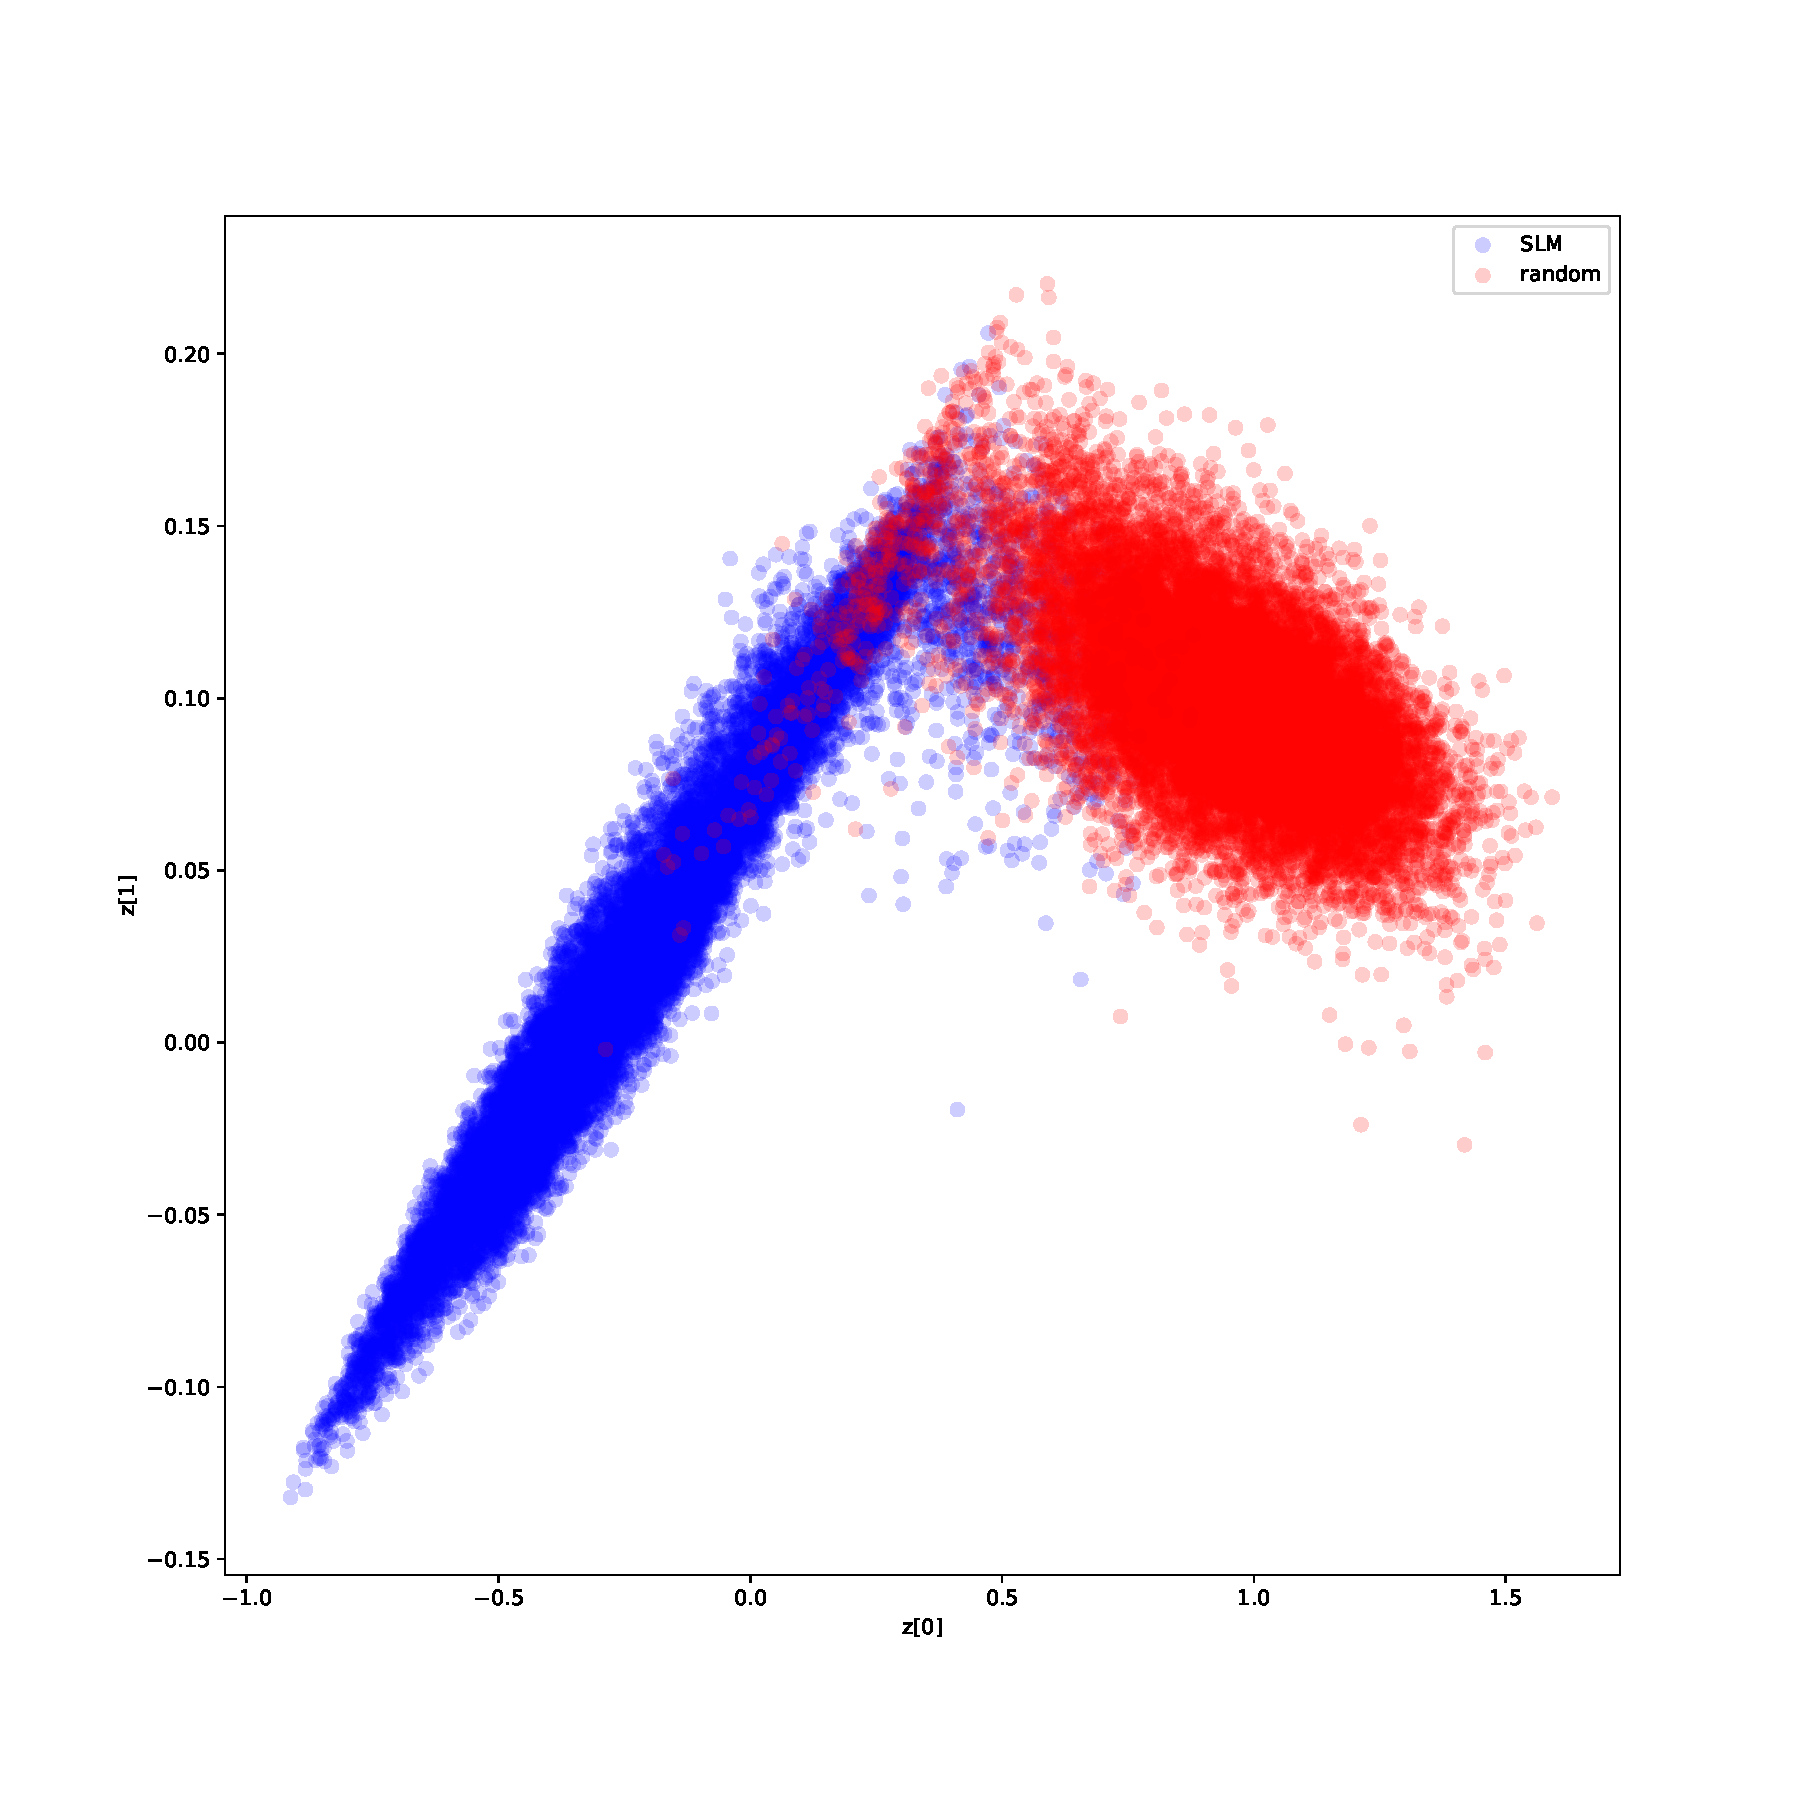
\includegraphics[scale=0.21]{vae_slm_all.pdf}
	\end{minipage}
	\caption{\it Image of clustered Standard like models. To the left with norm $V<5$. To the right all SLMs.}
\end{figure}
\end{frame}

\begin{frame}
\frametitle{Application: Clustering of SLM}
Clustering of SLMs
\bi
\item Compactification data is usually given in terms of integer matrices
\item SLM from heterotic on orbifolds {\color{blue} [1811.05993]}
\item SLM from $E_8 \times E_8$ on CICY {\color{blue} [2003.13339]}
\item SLM from $SO(32)$ on CICY {\color{blue} [2003.11880]}
\ei
\pause 
To do list:
\begin{enumerate}
\item Create data
\item Go down to two latent dimension to visualize
\item Find clusters of SLM
\item Profit.
\end{enumerate}
\end{frame}



\end{document}